\cotefile{36}
\scanpage{10}
% Brown two-stroke marginal mark: its interpretation as I), 1), or a bracket
% remains unresolved. The visible strokes are retained as a drawing.
\margin{\handwritten{\figure{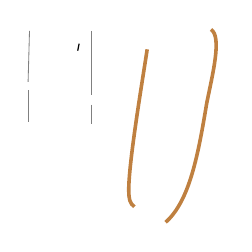
\begin{tikzpicture}[x=0.018cm,y=0.018cm]
\draw[gray,line width=.3pt] (-63,136) -- (-64,100);
\draw[gray,line width=.3pt] (-64,94) -- (-64,72);
\draw[gray,line width=.3pt] (-19,136) -- (-19,91);
\draw[gray,line width=.3pt] (-19,84) -- (-19,70);
\draw[black,line width=.45pt] (-28,127) -- (-29,122);
\draw[brown,line width=1.3pt] (20,123) .. controls (17,103) and (7,44) .. (7,24) .. controls (7,17) and (8,14) .. (11,12);
\draw[brown,line width=1.3pt] (65,137) .. controls (73,132) and (66,105) .. (62,85) .. controls (56,49) and (50,16) .. (33,1);
\end{tikzpicture}}}}
\handwritten{\uline{Le théorème de Griffiths par voie algébrique.}}

1.\quad Soit
\[
f:Y\handwritten{\longrightarrow}S
\]
un morphisme propre et lisse de schémas, avec $S$ \inserted{\handwritten{régulier,}} connexe à caractéristiques résiduelles toutes $\ne\unsure{\ell|\chi}$ (nombre premier fixé). Soit $s\handwritten{\in}S$, $\bar s$ un point géométrique au dessus de $s$. Soi\deleted{\unsure{t}}\handwritten{t} $F$ un faisceau $\ell$-adique constant tordu sur $S$ (en pratique, un faisceau de la forme $\underline{Z}_{\ell}(i)$ ), et $x$ une classe de cohomologie
\[
x\handwritten{\in}H^{\deleted{N}\handwritten{\unsure{m}}}(Y,\deleted{\unsure{f^*(F)|f^*F}}\handwritten{F_Y})\ .
\]
Disons que $x$ est \uline{primitive} si son image dans $H^0(S,R^m f_{\handwritten{*}}\handwritten{(\unsure{F|f}))}\deleted{(F))}$ est nulle, ou ce qui revient au même par le th. de spécialisation de la cohomologie, si son image dans $H^{\deleted{N}\handwritten{m}}(Y_{\bar s},F_{\bar s})$ est nulle. Alors la suite spectrale de Leray pour $f$ nous donne un élément
\[
u(x)\handwritten{\in}E_2^{1,\deleted{\unsure{N-1|m-1|N}}\handwritten{m-1}}=H^1(S,R^{\deleted{\unsure{m|N}}\handwritten{m-1}}_{\deleted{\unsure{2|f}}}f_{\deleted{\unsure{f}}\handwritten{*}}(F_{\handwritten{Y}}))\ .
\]
Donnons une propriété fonctorielle générale de cette classe $u(x)$. Pour ceci, soit $Y'$ lisse et propre sur $S$, et
\[
\unsure{Z|z}\handwritten{\in}H^N(Y\mathbin{\mathrm{x}}_S Y',G),
\]
de sorte que par le formalisme des correspondances cohomologiques, $z$ définit une application
\[
x'\handwritten{\longmapsto}Z(x'): \quad H^{m'}(Y',F')\handwritten{\longrightarrow}H^m(Y,F),
\]
si on suppose $m=m'+N-\handwritten{2}d^{\handwritten{\prime}}\deleted{\unsure{\mathrm{im}(Y'/S)|\mathrm{im}(X'/S)}}$, et qu'on a un accouplement $F'\mathbin{\text{\rlap{\kern.1em$\mathrm{x}$}\handwritten{$\bigcirc$}}}G\handwritten{\longrightarrow}F(d')$ (NB $d'$ est la dimension relative de $Y'$ sur $S$, supposée constante, et $(d')$ désigne le twist de Tate\deleted{\unsure{de|xx}}; $F'$ et $G$ désignent des faisceaux $\ell$-adiques constants tordus \inserted{\handwritten{sur $S$}} tout comme $F$). Ceci dit, si $x'$ est primitive, alors il en est évidemment de même de $x=Z(x')$, et on aura de plus
\[
u(Z(x'))=Z(u(x'))\ ,
\]
où le deuxième membre s'explicite en notant que $Z$ définit également, par
% archive sheet number: 9
